\chapter{Implementación}


\section{Controladores}

El controlador digital presentado en la sección \ref{cap3_controladores} se implementó en lenguaje C usando la transformada directa II.

%https://www.keil.com/pack/doc/CMSIS/DSP/html/group__BiquadCascadeDF2T.html


\subsection{Microcontrolador}



\subsection{Puente H}

Funciones especificas

\section{Integración de hardware}

Esquematico y componentes

\subsubsection{PCB}

Placa PCB

\section{Bus de campo}

Conexión


\section{Software}

\subsection{ROS}

Como se monstró en el capitulo pasado, su utilizó ROS como framework para realizar la integración. Los dispositivos de hardware, el robot Scorbot y el dispotivo háptico Phantom, cuentan con su \textit{nodo driver} que permiten la integración con el ecosistema ROS.

Se entiende por \textit{nodo driver} o ROS \textit{wrapper}, a una aplicación que actua como puente entre un dispositivo fisico y su representación en ROS, permitiendo interactuar de forma transparente con el dispositivo mediante el uso tópicos y servicios. Usualmente el \textit{nodo driver} hace uso de librerías proveidas por el fabricante o terceros para el manejo protocolos especificos del dispositivo. Por ejemplo, las siguientes aplicaciones cumplen esta función:

\begin{itemize}

\item \textit{ROSARIA}\cite{rosaria}: corresponde a una aplicación construido usando la librería \textit{Adept MobileRobots Robotics Interface for Applications} (ARIA), permite el control de robots móviles de las compañias Adept MobileRobots, MobileRobots Inc., y ActivMedia, por ejemplo el Pioneer 3-DX y 3-AT.

\item \textit{kinova-ros}\cite{kinova}: Es el driver oficial ofrecido por Kinova robotics para el uso de los robot manipuladores Jaco y Mico.

\end{itemize}

\subsubsection{Integración del robot Scorbot}

En esta sección se describirá la función de cada uno de los nodos que integran el software desarrollado para el control del robot Scorbot.

\begin{figure}[ht]
  \centering
  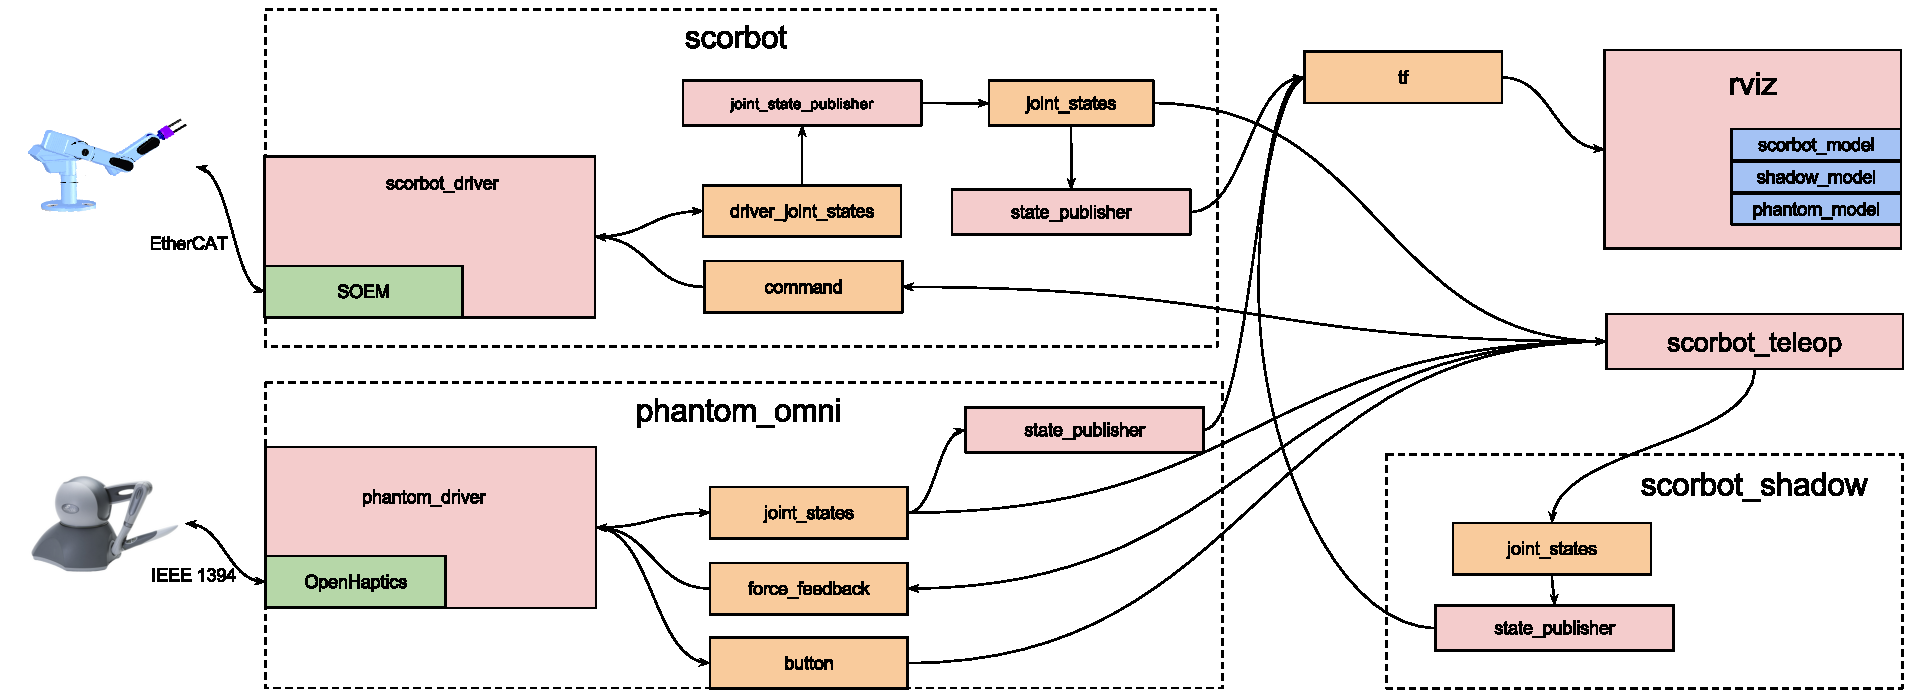
\includegraphics[width=\textwidth]{img/cap4/scorbot_software.pdf}
  \caption{Diagrama de nodos y tópicos de la aplicación.}
  \label{cap4_scorbot_software}
\end{figure}

\begin{description}

\item[\texttt{scorbot\_driver}] Corresponde al \textit{nodo driver} se integra con la librería SOEM \cite{soem} para la comunicación EtherCAT. Dado que este nodo ejecuta un ciclo de control, se consideraron una serie de requerimientos, muchos de ellos básicos para software de ejecución en tiempo real:

\begin{itemize}
\item Separación de hilos de ejecución, todas las tareas realacionadas con actualización de datos en el bus de control se realiza en un hilo independiente (\textit{control thread}) a las comunicaciones con el framework ROS (ROS \textit{thread}).
\item La comunicación entre el  \textit{control thread} y el ROS \textit{thread} se realiza usando estructuras de datos no bloqueantes.
\item La memoria utilizada por el hilo de control queda fija luego de la inicialización, de esta forma no se hacen llamados al sistema para pedir o liberar memoria.
\end{itemize}

SOEM mapea en memoria los dispositivos, es decir, desde el la aplicación master se tiene acceso a un buffer de memoria que permite leer y escribir en los dispositivos esclavos. Para obtener los datos manipulables, se debe usar la misma estructura de datos que usa el dispositivo esclavo para representar la información. \texttt{setpoint\_t} es la estructura usada como referenca (\textit{set point}), miestras que \texttt{joint\_data\_t} es la información del estado del controlador. Estas estructuras estan contenidas en un archivo de cabezera generado por el SSC, su modificación debe realizarse de forma cuidadosa, pues se pueden obtener errores de representación. El Código fuente \ref{cap4_estructuras} muestra la composición de ambas estructuras, notar el uso de la instrucción \texttt{PACKED}, que indica al compilador no añadir bytes entre los elementos de la estructura, de esta forma todos los elementos estan contiguos en memoria.

\begin{lstlisting}[language=C,style=csstyle, caption=Estructuras de datos usadas para mapear datos de dispositivos esclavos, label=cap4_estructuras]
typedef struct PACKED {
    uint16_t controlRegA;
    uint16_t controlRegB;
    int16_t  currentRef;
    int16_t currentLim;
    uint16_t pidCurrentKp;
    uint16_t pidCurrentKi;
    uint16_t pidCurrentKd;
} setpoint_t;

typedef struct PACKED {
    int16_t encPosition;
    int16_t encSpeed;
    int16_t current;
    uint16_t limits;
} joint_data_t;
\end{lstlisting}

Luego de realizar el mapeo en memoria, se creó la clase \texttt{ScorbotJointDriver}, encargada de representar cada controlador. Posee metodos para modificar la referencia y obtener el estado del controlador. Todos los controladores se agrupan en la clase \texttt{ScorbotHardwareInterface}, la cual abstrae las funciones del robót manipulador, como enviar una referencia a todas las articulaciones y detener todos los controladores. Es también encargada de ejecutar el ciclo de actualización de todos los controladores, este ciclo se ejecuta a \SI{1}{\kilo\hertz}.

ROS posee el paquete \texttt{ros\_control}, cuya función es facilitar la integración de dispositivos de control en ROS. De esta forma la clase \texttt{ScorbotHardwareInterface} hereda de \texttt{hardware\_interface::RobotHW} permitiendo la integración con \texttt{ros\_control}. El principal elemento utilizado de \texttt{ros\_control} correponde al \texttt{cotroller\_manager} una clase encargada de la comunicación entre \texttt{hardware\_interface::RobotHW} y tópicos ROS usando estructuras no bloqueantes en un hilo de ejecución independiente.

\begin{figure}[ht]
  \centering
  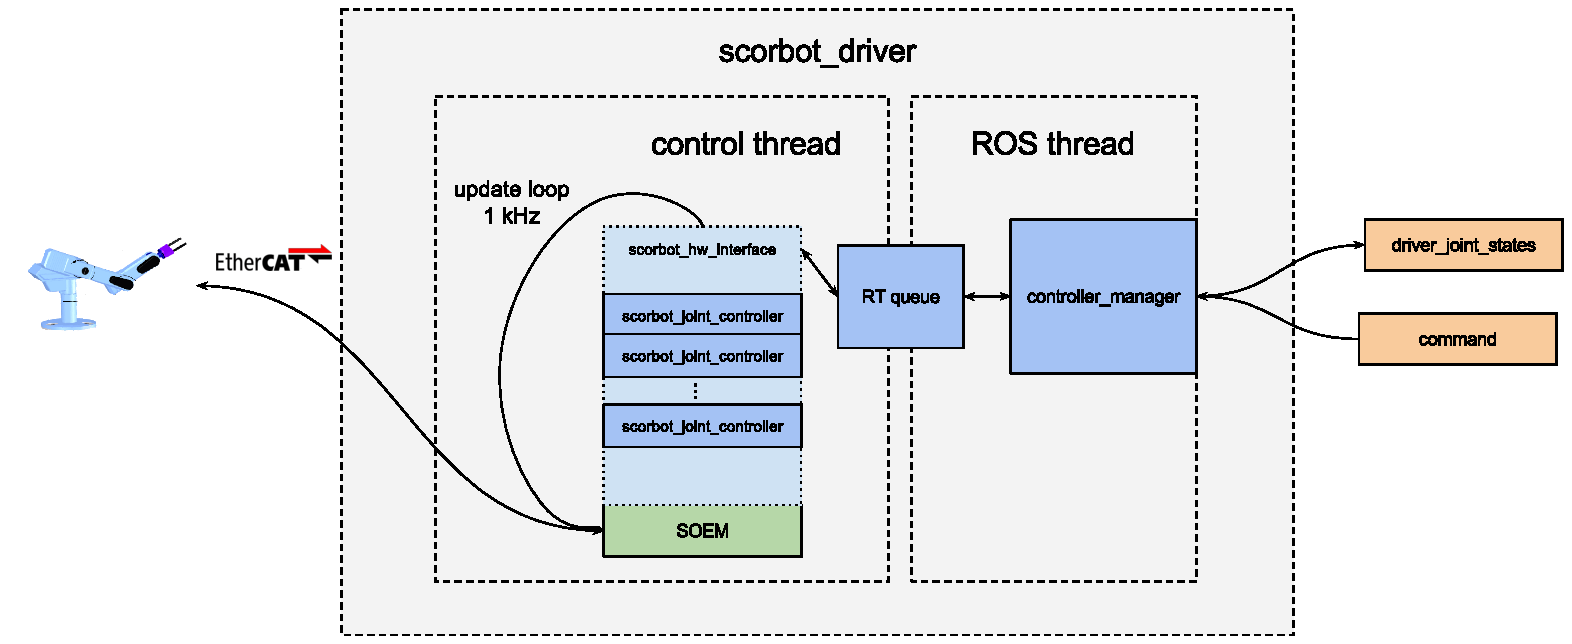
\includegraphics[width=\textwidth]{img/cap4/scorbot_driver.pdf}
  \caption{Diagrama del nodo \texttt{scorbot\_driver}.}
  \label{cap4_scorbot_driver}
\end{figure}

La Figura \ref{cap4_scorbot_driver} muestra la estructura del nodo \texttt{scorbot\_driver} como se ha señalado anteriormente. Como se ha mensionado anteriormente, es el \texttt{controller\_manager} quien se encarga de la comunicación con ROS, usando distintos tópicos:

\begin{itemize}

\item \texttt{driver\_joint\_states}: Contiene la información sobre el estado de cada articulación: posición, velocidad, aceleración y tiempo. Usa el mensaje  \texttt{sensor\_msgs/JointState[]}.

\item  \texttt{command}: Se usa para obtener la referencia de posición que será enviada a los controladores, se usa el mensaje \texttt{std\_msgs/Float64[]}.
 
\end{itemize}



\item[\texttt{joint\_state\_publisher}] Corresponde a un nodo estándar de ROS, cuya función es obtener los estados de las articulaciones de distintas fuentes (tópicos) y publicarlos de forma conjunta, completando el estado de todas las articulaciones dependiendo de la descripción del robot (URDF).

\item[\texttt{robot\_state\_publisher}] Corresponde a un nodo estándar de ROS, es el encargado de tomar la información de las articulaciones del robot y publicar el árbol de transformadas de cada uno de los enlaces del robot basado en la descripción del robot (URDF), es decir, ejecuta la cinemática directa del robot. Esta información de las transformadas es publicada en el tópico \texttt{/tf}.

\end{description}


\subsubsection{Integración de la interfaz Phantom Omni}

En esta sección se describirá la integración del dispositivo Phantom Omni en ROS. En este caso se hace uso del paquete \textit{phantom\_omni}\cite{phantom_git}, que contiene el ROS wrapper y URDF. La integración del Phantom Omni en ROS es similar a la realizada con el robot Scorbot, pues cuenta con el  ROS wrapper y los nodos \texttt{robot\_state\_publisher} y  \texttt{joint\_state\_publisher}, que cumplen la misma función descrita anteriormente, salvo que actúan sobre el estado del Phantom Omni.

\texttt{phantom\_driver} Corresponde al \textit{nodo driver} se integra con la librería OpenHaptics para la comunicación con dispositivo Phantom Omni a través de FireWire. Provee los siguientes tópicos:

\begin{itemize}
\item \texttt{joint\_states}: Información sobre el estado de las articulaciones usando el mensaje \\ \texttt{sensor\_msgs/JointState[]}.

\item \texttt{button}: Información sobre el estado de los botones del stylus del Phantom Omni, usando el mensaje \texttt{omni\_msgs/OmniButtonEvent}.

\item \texttt{force\_feedback}: El nodo se suscribe a éste tópico, al publicar en él el dispositivo aplica un par sobre las articulaciones actuadas.
\end{itemize}

Todos los tópicos del \texttt{phantom\_driver} se ejecutan a una frecuencia de \SI{100}{\hertz}, esto asegura que la referencia y retroalimentación hacia el operador sea adecuada, en terminos de retardo.


\subsubsection{Teleoperación}

La aplicación encargada de la teleoperación debe, básicamente, conectar el robot Scorbot con la interfaz háptica Phantom Omni, por conectar se entiende que la aplicación realiza el mapeo de las articulaciones del Phantom Omni hacia las articulaciones del Scorbot y entrega retroalimentación usando el Phantom Omni. Esta tarea es realizada por el nodo \texttt{scorbot\_teleop}.

El nodo \texttt{scorbot\_teleop} no controla directamente al robot Scorbot, si no que a un robot virtual, denominado Scorbot \textit{shadow}, esta representación almacena la posición deseada para el robot. Uno de los botones del \textit{stylus} del Phantom Omni actúa como gatillo, enviando la referencia es enviada al robot. Si el usuario mantiene el botón presionado, el software enviará de manera continua (\SI{100}{\hertz}) la referencia al robot.

\begin{figure}[H]
  \centering
  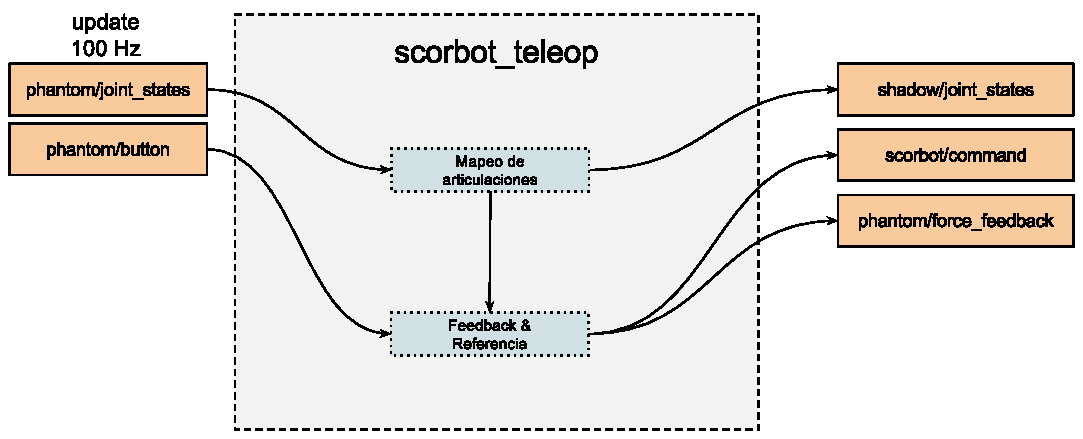
\includegraphics[width=0.8\textwidth]{img/cap4/scorbot_teleop.pdf}
  \caption{Diagrama del nodo \texttt{scorbot\_teleop}.}
  \label{cap4_scorbot_teleop}
\end{figure}

La Figura \ref{cap4_scorbot_teleop} muestra funcinamiento interno del nodo \texttt{scorbot\_teleop}, el mapeo entre el Phantom y el Scorbot \textit{shadow} se realiza de forma continua con propósitos de visualización. La retroalimentación hápica es calculada a partir de la differencia en la posición del Scorbot \textit{shadow} y el robot real, dado que ambos dispositivos tienen una morfología similar y poseen el mismo número de grados de libertad, el cálculo se realiza la ley de Hooke \cite{handbook}, donde la posición corresponde a la posición de las articulaciones, como se indica en la Ecuación \ref{cap4_hooke}.

\begin{equation}\label{cap4_hooke}
F_i = K_i({X_{shadow}}_i - {X_{scorbot}}_i) \, \mbox{con } i \in {1,2,3}
\end{equation}

Donde $K_i > 0 \, \mbox{con } i \in {1,2,3}$. Notamos que el cálculo solo considera en las primeras tres articulaciones, pues el Phantom Omni solo posee tres articulaciones actuadas. En el Scorbot, las últimas dos articulaciones se encuentran cercanas al efector y definen su orientación, por lo que son las tres primeras articulaciones las que tinen el rol principal en definir la posición del efector.

\subsubsection{Visualización}



\texttt{rviz}

\texttt{scorbot\_shadow}


\subsubsection{Modelo URDF}

El modelo \textit{Unified Robot Description Format} (URDF) es un formato basado en XML (\textit{Extensible Markup Language}), corresponde al estandar para la representación de robots en el framework ROS. Para crear 

\begin{figure}[H]
  \centering
  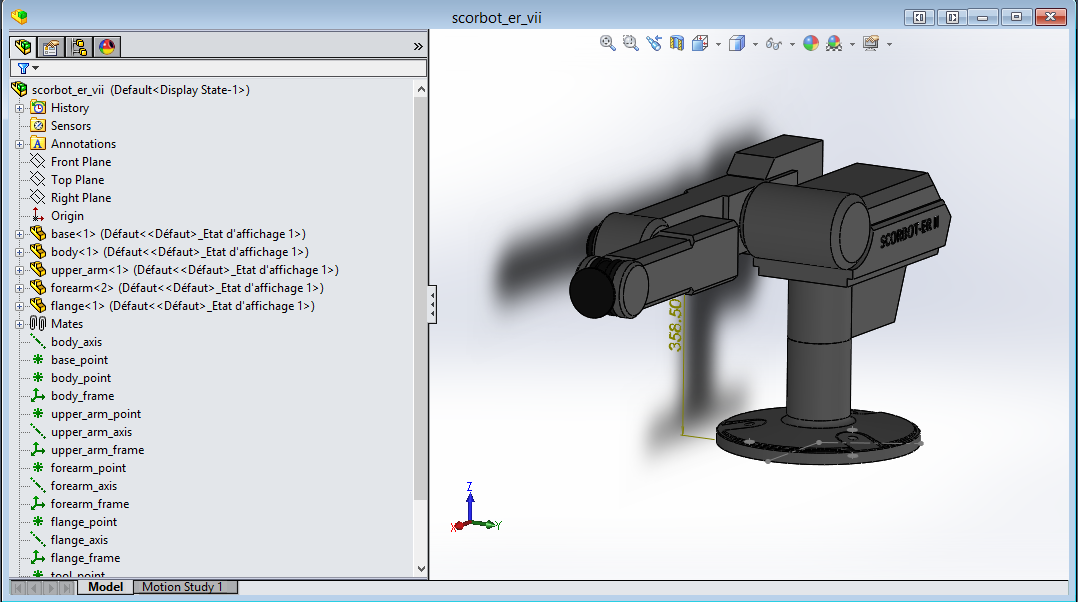
\includegraphics[width=0.8\textwidth]{img/cap4/cad_solidworks.PNG}
  \caption{Modelo del robot Scorbot en SolidWorks.}
  \label{cap4_scorbot_cad}
\end{figure}



